\section{Curve25519 Key Exchange}\label{curve25519-key-exchange}

\emph{Author of section and module: Andres Erbsen.}\\As classical
Diffie-Hellman-Merkle key-exchange requires hundreds of modular
arithmetic operations on multiple-thousand-bit numbers to be secure, we
will be using a modern variation where every modular multiplication is
replaced with the addition of two points on a carefully chosen elliptic
curve{[}@Curve25519{]}. The other relevant properties of elliptic curve
addition are the same as for modular multiplication, so we will continue
to use the classical notation. Even though one elliptic curve addition
uses 10 modular multiplications, the same level of security can be
achieved using numbers that are 10 times shorter. Numbers that are 10
times shorter are 100 times easier to multiply, leading to 10 times less
chip area and time usage.

The elliptic curve cryptography implementation is the most technically
involved part of this project. The paper that introduced
Curve25519{[}8{]} gives explicit formulas for the elliptic curve
arithmetic in terms of operations on integers modulo the prime
\(p=2^{255} -19\). Our implementation of the Curve25519 module follows
the figure presented in the appendix of that paper and makes use of the
properties of our modular arithmetic modules to provide better
performance. The main computation consists of 255 iterations of the
elliptic curve Montgomery ladder step operation, each of which involves
10 modular multiplications and a couple of additions and subtractions.
To allow for a simpler and faster implementation, the intermediate
results are stored as fractions and the final output fraction is reduced
to a scalar at the very end, requiring modular division. To save area,
the circuit has only one copy of the modular multiplication unit and one
add/subtract unit; these are used in sequence to compute the elliptic
curve operation and the division. Furthermore, as the latency of our
modular multiplication unit is twice as high as the latency of the
addition/subtraction unit, but the throughput is the same, we did our
best to keep the multiplication pipeline active at all times. This
results in using 7 255-bit registers to store the intermediate values,
in addition to the internal registers of the modular arithmetic units.
All in all, our implementation requires less than 70000 cycles to
perform an elliptic curve operation (public key generation or shared key
generation). Our implementation is a trade-off between speed, circuit
area, and complexity. We believe that more careful pipeline management
could offer slightly better speeds for any area, storing the
intermediate values of the elliptic curve operations in block RAM
instead of registers would allow for a smaller area at the expense of
speed, and implementing a dedicated modular division (inversion) unit
would allow for significantly better performance at even larger expense
of area.

\subsection{Modular multiplication}\label{modular-multiplication}

We took advantage of the fact that the modulus (\(p=2^{255}-19\)) was
known at the design time, that it is very close to a power of two, and
the availability of 18-by-18-bit multipliers to create implement an
efficient modular multiplication unit. The overall strategy is depicted
in the following figure.

\begin{figure}
\label{figFemul}
\makebox[\textwidth][c]{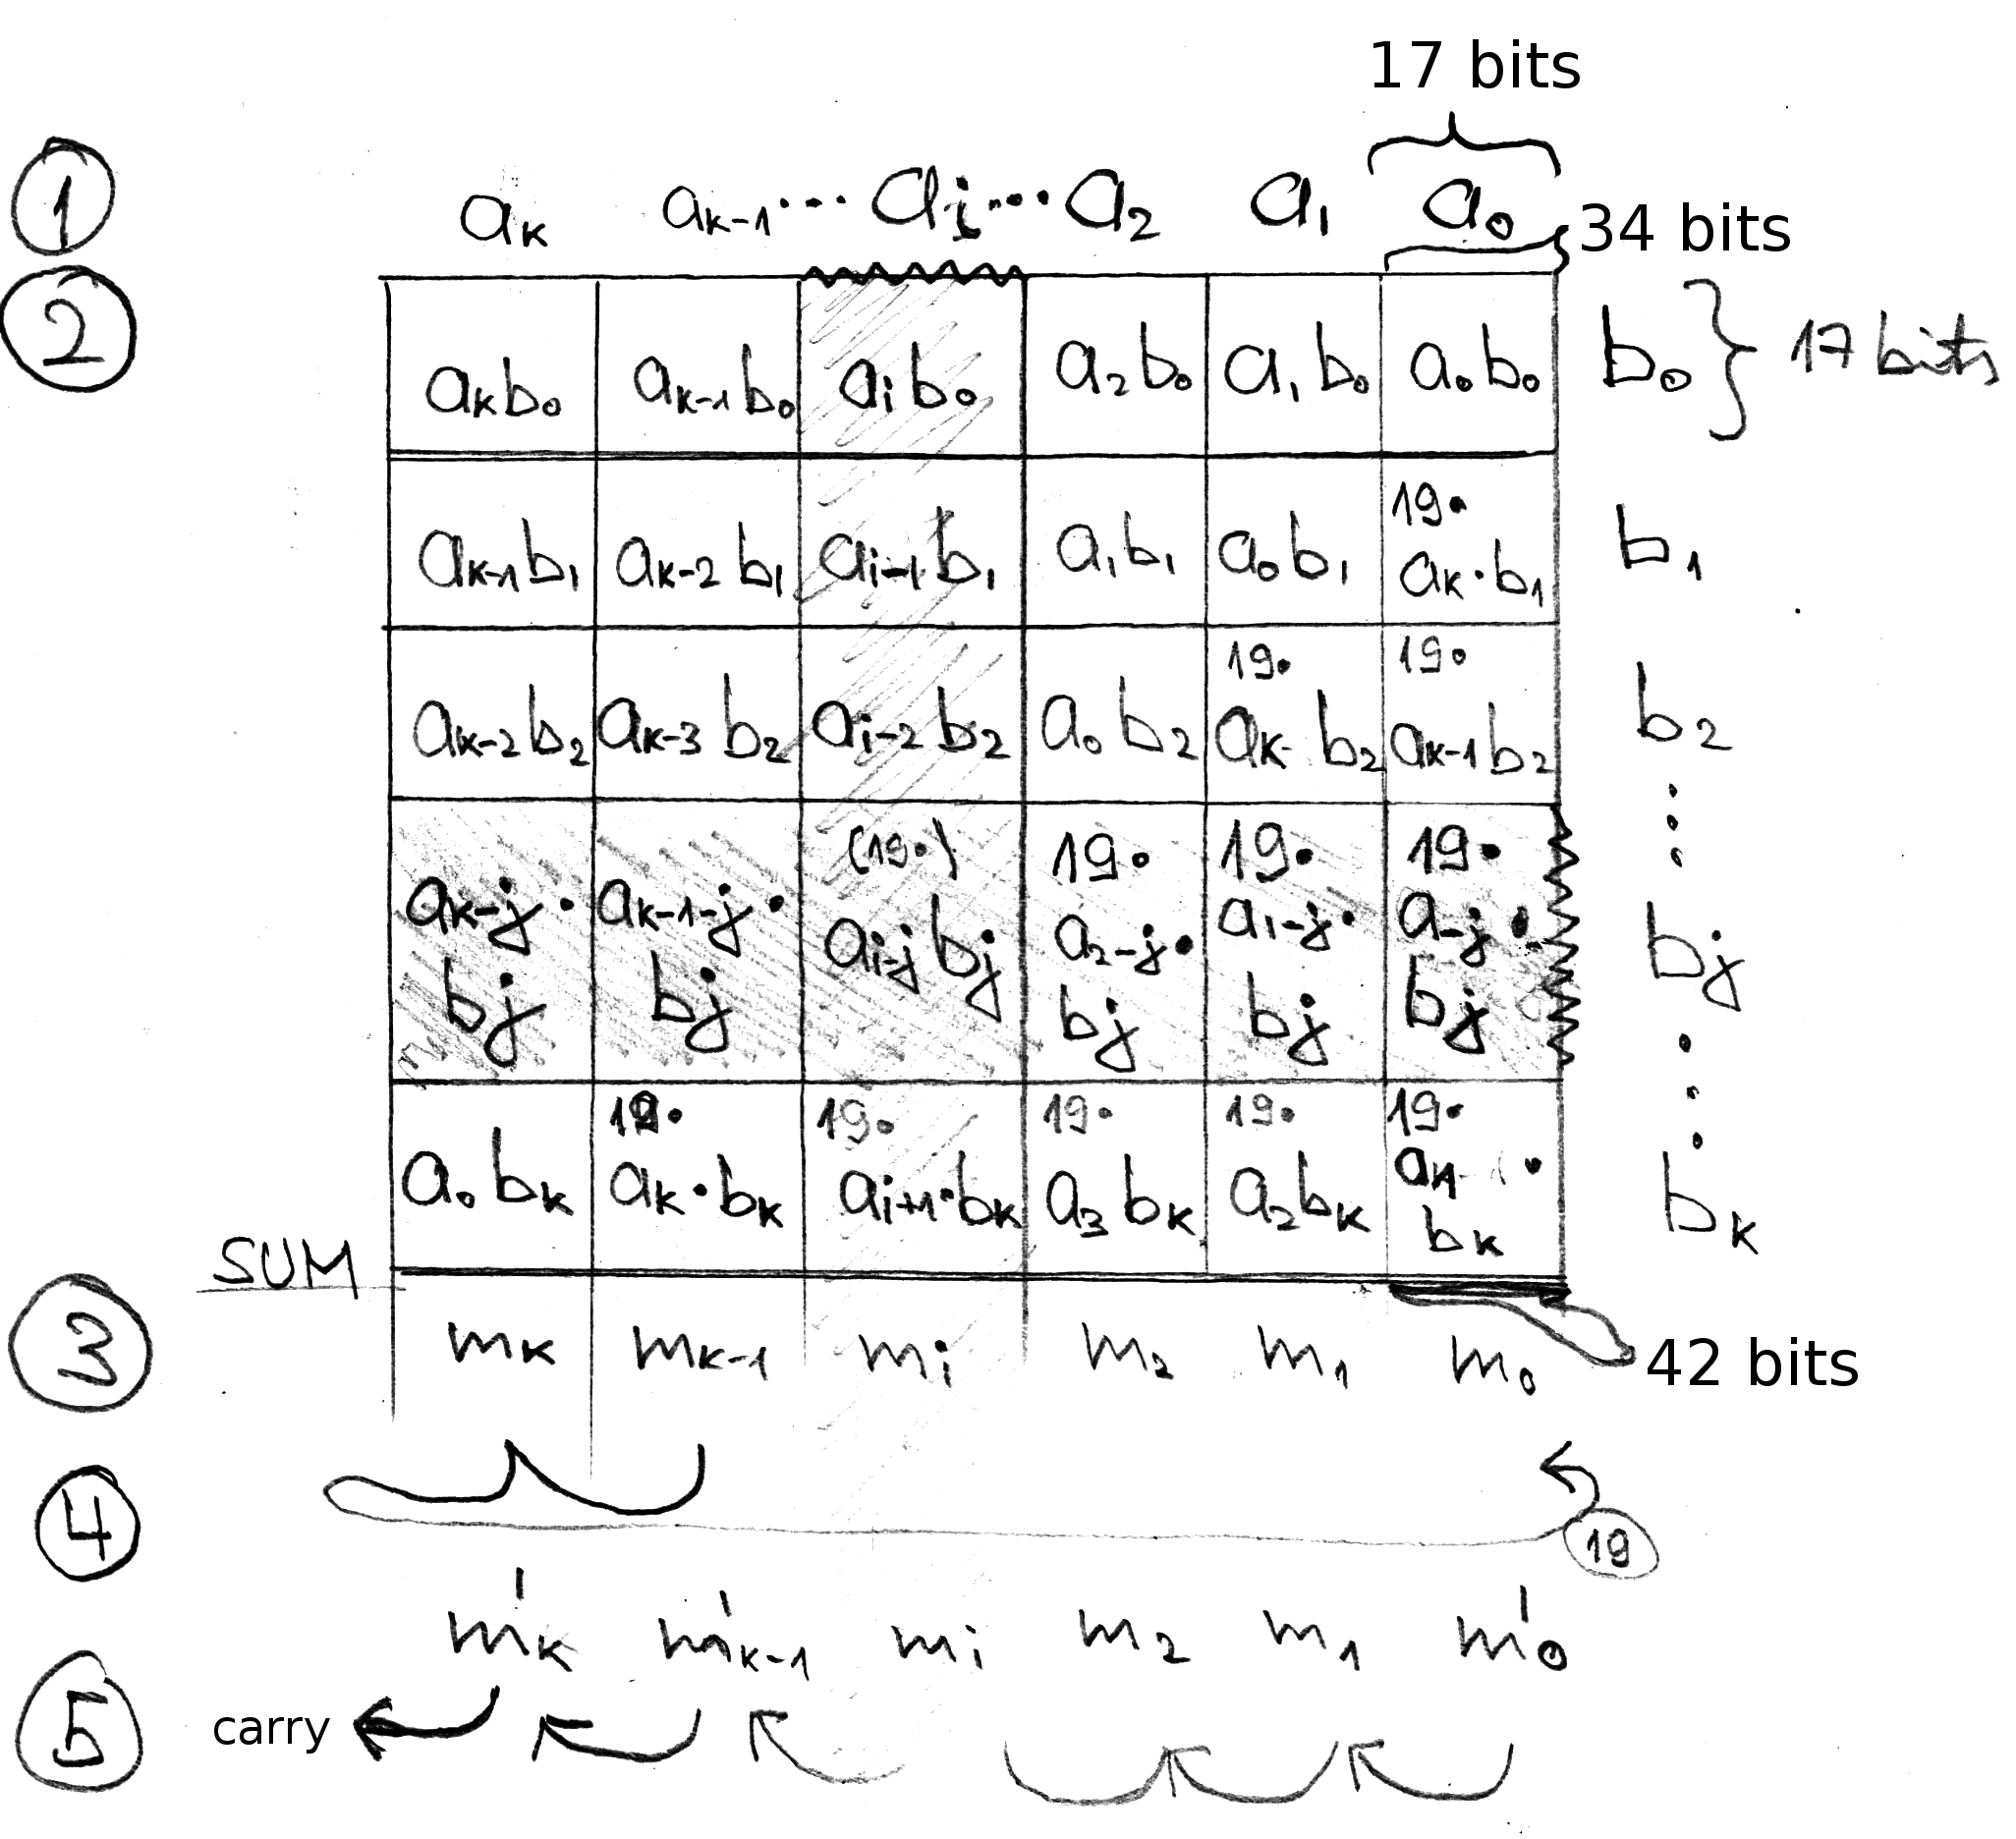
\includegraphics[width=\textwidth]{figs/femul.png}}%
\centering \caption{Overview of modular multiplication of $255$-bit integers $a$
and $b$. $a_0$ is the least significant 17-bit digit of $a$. Each row of the
table in step 3 is computed in 1 clock cycle.}
\end{figure}

\begin{enumerate}
\def\labelenumi{\arabic{enumi}.}
\itemsep1pt\parskip0pt\parsep0pt
\item
  Interpret each 255-bit input as 15 17-bit digits. While it would have
  been possible to use 18-bit digits, choosing 17 greatly simplifies the
  implementation because 255 bits can be evenly divided into 17-bit
  digits but not into 18-bit digits.
\item
  Perform an algorithm similar to schoolbook multiplication, where

  \begin{itemize}
  \itemsep1pt\parskip0pt\parsep0pt
  \item
    During each clock cycle, one row of partial products is computed
  \item
    Each partial product that would eventually overflow the 255-bit
    result because of its position is omitted from the calculation.
  \item
    However, the overflowing partial product is not discarded. As the
    modulus is \emph{not} a power of two, correct for the difference
    between two's complement integer overflow and addition mod \(p\) by
    adding 19 times the number of times the overflow wrapped around to
    the result. Because there must be an empty low order partial product
    slot for each partial product that is statically known to overflow,
    no addition needs to be performed: the just system places 19 times
    the overflowing partial product to the correct slot.
  \end{itemize}
\item
  Cumulatively add up the columns of partial products, but do not handle
  carries between them. The sum of each column has an upper bound of 42
  bits because it is a sum of 17 products of two 17-bit numbers times
  19.
\item
  Handle carries from the two most significant columns, adding the
  number of overflows times 19 to the result as before.
\item
  Handle all remaining carries starting from the least significant
  column and moving towards towards the most significant column. The
  result will be between \(0\) and \(2p\).
\item
  If the result overflows (has a carry of 1), subtract \(p\) from it.
  This is \emph{not} implemented as a separate step. Instead, there are
  two copies of steps 4 and 5, one of which works as described and the
  other subtracts the appropriate digit of \(p\) while handling each
  carry. The correct output is selected amongst the two branches using
  the carry bit.
\end{enumerate}

The breakdown of time usage is roughly as follows: step 2 takes 17
cycles, step 4 takes 1 cycle, and step 5 takes 17 cycles. As the FPGA
provides fast 17-by-17-bit multipliers in dedicated silicon, the main
area usage is due to the the accumulator and operand registers, and the
42-bit adders used for adding up columns and propagating carries.

\subsection{Modular Addition and
Subtraction}\label{modular-addition-and-subtraction}

Addition and subtraction also operate on 15 17-bit digits. While a
larger digit size would have offered superior speed at the submodule
level, we chose to stay consistent with the multiplier implementation
because the addition and subtraction latency is currently not the
bottleneck in the overall system. The general algorithm closely follows
the schoolbook method, and can also be seen as a ripple-carry adder
where a 1-by-1-bit ``full adder'' is replaced with a 17-by-17-bit digit
adder. As in multiplication, we need to ensure that the result of the
operation wraps modulo \(p=2^{255}-19\). Unlike multiplication, the
carry (resp. borrow) can only be a single bit, so there is no need for
special handling of carries from higher digits. This allows us to
implement a modular addition (resp. subtraction) of the inputs \(a\) and
\(b\) by first computing both \(a+b\) and \(a+b-p\) (resp. \(a-b\) and
\(a-b+p\)) and selecting the one which is in the valid range to output
when the final carry (resp. borrow) bit becomes available.

Currently our system has separate circuitry for addition and
subtraction, but only one of them is used at once. We believe that it
would be possible to save some circuit area at negligible speed cost by
having one circuit that allows the operation to be indicated using an
input.

\subsection{Modular Inversion
(Division)}\label{modular-inversion-division}

Our system computes \(\frac{b}{a}\) as \(b\cdot\frac{1}{a}\).
Calculating \(\frac{1}{a}\) is implemented through exponentiation and
multiplication by Fermat's little theorem (\(a^{p-2} = a^{-1}\) mod p),
and exponentiation is done as repeated squaring and multiplication:
\(x^n= x \, ( x^{2})^{\frac{n - 1}{2}} \mbox{ if } n \mbox{ is odd, otherwise } (x^{2})^{\frac{n}{2}}\).
While we are aware of more complicated methods that allow to perform
modular inversion faster, we chose this one because it requires almost
no additional circuit area. Currently, modular inversion accounts for
one fifth of the total modular multiplications and one fourth of the
running time (because the ladder step is pipelined and inversion is
not).

\section{ChaCha20 Stream Cipher}\label{chacha20-stream-cipher}

\emph{Author of section and module: Andres Erbsen.}\\ChaCha20 is a
modern stream cipher. Given a secret key, it provides fast random access
to different positions of \(2^{130}\)-byte keystream which is XOR-ed
with the data to encrypt it. The procedure to compute a 64-byte block of
keystream consists of 20 rounds, each of which mutates a 4-by-4 table of
32-bit words by applying the \emph{quarter round} function to all
columns or all diagonals. A quarter round takes 4 32-bit inputs and
produces 4 32-bit outputs, mixing the bits of the input using addition,
rotation and XOR. Our circuit has four instantiations of the quarter
round module, and one of the twenty rounds is completed each clock
cycle. Finally, the output is computed by adding the initial table
entries to the final table entries (round 21 in our implementation).

This implementation provides good performance (3 bytes/cycle), but the
propagation delay of the circuit is rather large, limiting us to clock
frequencies under 50MHz. In our case it was not an issue (we are using a
27MHz), but a higher frequency implementation would probably need to
pipeline the quarter round function.

\section{Keccak hash function}\label{keccak-hash-function}

\emph{Author of section: Andres Erbsen.}\\We used an open-source Keccak
implementation by Homer Hsing, available at \texttt{opencores.org}. The
input is sent to the Keccak module in chunks of 1 to 4 bytes, the output
is a 512-bit high-quality pseudo-random blob generated as a function of
the input. The implementation we used advertises a speed of 2.4Gbit/s at
100MHz, but we used it at a much slower rate (less than 1Mbit/s).
